\documentclass[12pt]{article}


\usepackage{scicite}
\usepackage{hyperref}
\usepackage{graphicx}
\usepackage{caption} 
\usepackage{subfigure}
\usepackage{float}
\usepackage{amsmath}
\usepackage{amssymb}
\usepackage{times}


\topmargin 0.0cm
\oddsidemargin 0.2cm
\textwidth 16cm 
\textheight 21cm
\footskip 1.0cm



\newenvironment{sciabstract}{%
\begin{quote} \bf}
{\end{quote}}



\renewcommand\refname{References and Notes}


\newcounter{lastnote}
\newenvironment{scilastnote}{%
\setcounter{lastnote}{\value{enumiv}}%
\addtocounter{lastnote}{+1}%
\begin{list}%
{\arabic{lastnote}.}
{\setlength{\leftmargin}{.22in}}
{\setlength{\labelsep}{.5em}}}
{\end{list}}


% Include your paper's title here

\title{Deep speech} 


\author
{Vincent R\'ebiscoul, St\'ephane Pouget and Florent Gu\'epin}

% Include the date command, but leave its argument blank.

\date{}



%%%%%%%%%%%%%%%%% END OF PREAMBLE %%%%%%%%%%%%%%%%



\begin{document} 

% Double-space the manuscript.

\baselineskip24pt

% Make the title.

\maketitle 



% Place your abstract within the special {sciabstract} environment.

\begin{sciabstract}
  This document present our project in machine learning. We have implemented a voice recognition system i.e. our program is able to recognize spoken language and translate into text by computers.
 We use python3, Keras and Tensorflow.
\end{sciabstract}



\section*{Introduction}

We have implemented this article \cite{article} with python3, Keras and Tensorflow. The neuralx network used is not common. So we created our own neural network model.

\section{Model}

\subsection{Topology of the model}

We have seven layers of neuron. The three first layers are computed by :

\[ h_t^{(l)} = g(W^{(l)}h_t^{(l-1)} + b^{(l)}) \]

where $g(z) =$ min\{max $\{0,z\}, 20\}$ and $W^{(l)}, b^{l}$ are the weight matrix and bias parameters for layers $l$.

The fourth layer is a bi-directional reccurent layer. This layer includes two sets of hidden units : a set with forward reccurence, $h^{(f)}$, and a set with backward recurrence $h^{(b)}$ : 

\[ h_t^{(f)} = g(W^{(4)}h_t^{(3)} + W_r^{(f)}h_{t-1}^{(f)} + b^{(4)}) \]

\[ h_t^{(b)} = g(W^{(4)}h_t^{(3)} + W_r^{(b)}h_{t+1}^{(b)} + b^{(4)}) \]

The fifth (non-recurrent) layer takes both the forward and backward units as inputs $h_t^{(5)} = g(W^{(5)}h_t^{(4)} + b^{(5)} $ where $h_t^{(4)} = h_t^{(f)} + h_t^{(b)}$. The output layer is a standar softmax function that yields the predicted character probabilities for each time slice $t$ and character $k$ in the alphabet :

\[ h_{t,k}^{(6)} \equiv \mathbb{P}(c_t=k | x) = \frac{exp(W_k^{(6)}h_t^{(5)} + b_k^{(6)})}{\sum_j exp(W_j^{(6)}h_t^{(5)} + b_j^{(6)})} \]


\begin{figure}[H]
  \begin{center}
    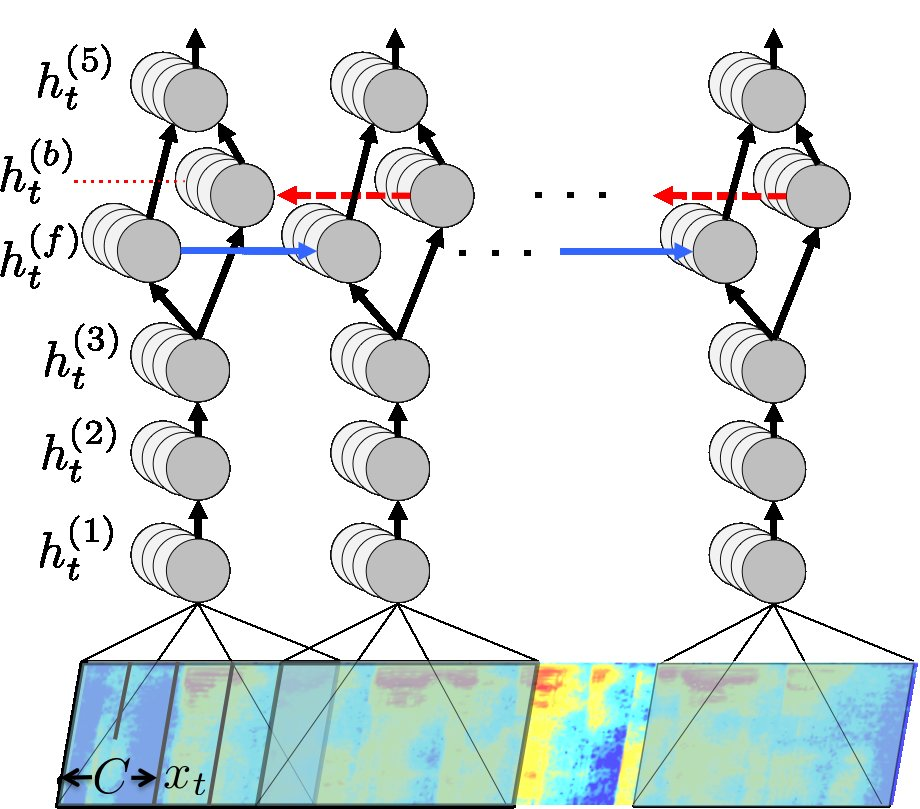
\includegraphics[scale=0.20]{images/photo.jpg}
    \caption{Structure of our RNN model}
  \end{center}
\end{figure}

\subsection{Analysis of the model}
The model we use is a Recurrent Neural Network (RNN), the particularity of a recurrent neural network is that recurrent layer has a state and for to compute the value of a time slice, the layer can take the output value of the same layer one step before or one step after. In our case, we have two recurrent layers, with $h_t^f$ depends on $t-1$ (so $h_t^f$ depends on what happened previously). $h_t^b$ depends on $t+1$ so it depends on what will happen next. The idea is that we cannot link a sound to a letter without putting it in context. For example, in the word "the", our neural network cannot predict that the first letter is t because t has several pronounciation depending on the letter preceding of following. This is why we need two recurrent layers, one with a forwad recurrence and one with a backward recurrence.


\section{Our work}

\subsection{The implementation of the model}

This article \cite{article} create a new model and use a ctc loss function. So to create this model, we have customized our model so that it is like on the article. For that we had to work a lot on the documentation of keras and tensorflow. However our main problem was the ctc loss function. At the beginning, we had troubles to understand how the backend function ctc\_batch\_ cost worked. First, one has to know that the CTC loss function is very peculiar. Indeed, our neural network slices an audio file in several time slices and then for each time slice, it tries to predict which letter it is. Now, suppose you give a recording of someone saying the expression ``good morning''. If the neural network is correctly trained, it should output something like ``gggoooodd moorrnnninng'' (there are several time slices corresponding to the same letter), thus the cost $\mathcal{L}(\mbox{good morning}, \mbox{gggoooodd moorrnnninng})$ should be small when the cost $\mathcal{L}(\mbox{good morning}, \mbox{good mornint})$ should be higher. This makes the CTC function essential but complicated. Another problem is that the ctc\_batch\_cost function takes four parameters, but in Keras, the loss function only takes 2 parameters. To avoid this problem, we had to create a new lambda layer which outputs the loss of the batch and is connected to several other layers which feeds the different arguments that are needed. Apparently, this is a known trick in Keras to avoid a common problem.

\subsection{The dataset}

The dataset that we used is not composed of sentences or expressions but of words. The idea was to have easily trainable neural network that could work quickly and would be able to recognize at least some words. Indeed, in the article they say they managed to have a solid working neural network but using several optimisations and with 5000 hours of training. This seemed too much for machine learning rookies. Obviously this makes a neural network weak when you train it on sentences but it works better on words (at least the words where the neural network has been trained on).

\bibliography{scicite}

\bibliographystyle{Science}

\end{document}
